\documentclass[10.5pt,twocolumn]{aaas}

%%画圆圈数字
\newcommand*\circled[1]{\tikz[baseline=(char.base)]{\node[shape=circle,draw,inner sep=1pt] (char) {#1};}}
            
\newcommand\mycolorRed[1]{{\color{red}#1}}
\newcommand\mycolorYellow[1]{{\color{yellow}#1}}
\newcommand\mycolorBlue[1]{{\color{blue}#1}}

\DeclareMathSizes{10.5}{10}{6.8}{4.2}

\setlength{\abovedisplayskip}{2.5mm}
\setlength{\belowdisplayskip}{2.5mm}

\usepackage{tabu}
\usepackage{longtable}
\usepackage{makecell}
\usepackage{multirow}
\renewcommand\cellgape{\Gape[-3pt][-3pt]}

\usepackage{dashrule}
\usepackage{newtxmath}
\usepackage{stfloats}

\begin{document}
\title{
\xiaoerhao\textbf{基于光流跟踪与自适应运动补偿的视频防抖算法研究} \vspace{0.4cm}
}

\author{
\sihao 马子昂 \makebox{$^{\text{1, *}}$}，蔡建宇 \makebox{$^{\text{1}}$}，石兴霖 \makebox{$^{\text{1}}$}，陆冲 \makebox{$^{\text{1}}$}，黄俊源 \makebox{$^{\text{1}}$}，马明义 \makebox{$^{\text{1}}$}，刘琪瑞 \makebox{$^{\text{1}}$}，聂方凯 \makebox{$^{\text{1}}$}\\[0.3cm]
\xiaowuhao 1.~~中国民航大学~~计算机与人工智能学院，天津~~300300\\ 
}

\date{}

\CKeyword{视频防抖； KLT光流跟踪； 相似变换； RANSAC； L1最优路径； 自适应裁剪； 时域运动补边}
\CLCNo{TP0001}
\Dcode{A}
\PaperNo{1001-1001 （2026） 01-0000-00}

\twocolumn[
  \begin{@twocolumnfalse}
  \maketitle
%\positiontextbox{2.25cm}{3.24cm}{\ArialFont \xiaowuhao http://hkxb.buaa.edu.cn \quad  hkxb@buaa.edu.cn\\}
%\positiontextbox{2.25cm}{4.3cm}{
%\liuhao 
%\parbox{\textwidth}{%
%{\CJKfontspec[FakeSlant = 0.2]{STHeiti}  引用格式:}{ \CJKfontspec[FakeSlant = 0.2]{STSong} 张某, 吕某某, 诸葛某, 等. 基于VLFeat与维纳去卷积的视频运动防抖算法研究\textsl{[J]}. 航空学报, \textsl{2026, 38(x): XXXXXX. ZHANG M, LYU M M, ZHU M,\\[-0.5em]
%\hphantom{引用格式:} et al. Research on Video Stabilization Algorithm Based on VLFeat and Wiener Deconvolution[J]. Acta Aeronautica et Astronautica Sinica, 2026, 38(x): XXXXXX(in Chinese). doi:}}
%}}
\begin{CAbstractAAAS}
视频稳定是无人机侦察、手持摄像等计算机视觉领域的重要研究课题。针对实际录像中摄像机高频随机抖动导致主观体验下降并干扰后续视觉任务的问题，本文提出了一个不依赖深度学习、可近实时运行的三阶段模块化视频防抖流水线。本文最初尝试了自主研发的帧间光流与角点检测代码，但因特征跟踪精度有限、对前景动态外点干扰敏感而效果不佳。为此，本文基于 OpenCV~\cite{bradski2000} 的 C++ 高效后端重构流水线：运动估计阶段采用降采样 Shi-Tomasi 角点~\cite{shitomasi1994} 与金字塔 KLT 光流~\cite{lucas1981,bouguet2001} 跟踪，辅以前向-后向一致性校验~\cite{kalal2010} 剔除不可靠点，并用 RANSAC~\cite{ransac1981} 拟合 4 自由度相似变换以稳健覆盖平移、旋转与缩放；运动平滑阶段先以矩阵连乘累积绝对轨迹，再分解到平移、旋转角与对数尺度参数空间，分别采用零相移高斯低通与 L1 最优相机路径~\cite{grundmann2011} 两种平滑器分离主动运动与抖动；帧合成阶段提出预算约束下的自适应中心裁剪与全幅时域运动补边~\cite{matsushita2006} 两种去黑边策略，并以 USM 锐化补偿插值损失。实验在手持步行、骑行颠簸、画面剧烈抖动与静止站立四种带真值的合成抖动场景下进行：运动估计的平移均方根误差（RMSE）介于 12.59 至 48.66 像素之间，有效防抖时长占比由处理前的 0.6\%--49\% 提升至 56\%--96\%（仅极端骑行颠簸工况例外），平均逐帧抖动由 7--9 像素降至约 1 像素，运动估计平均约 3--7\,ms/帧，兼具良好的实时性与工程实用价值。
\end{CAbstractAAAS}
%%%%%%%%首页角注
%\positiontextbox{2.2cm}{25.2cm}{
%\noindent\hdashrule{7.5cm}{0.6pt}{2.5pt 0.8pt}\\[3.5ex]%
% \liuhao \linespread{0.8}\selectfont
%\parbox{\textwidth}{%
%makebox[\widthof{\makebox{*}收}][r]{收}稿日期: 2026-06-01； 录用日期： 2026-xx-xx； 网络出版时间：2026-xx-xx； \\%
%\makebox[\widthof{\makebox{*}收}][r]{网}络出版地址: http://hkxb.buaa.edu.cn/CN/html/2026XXXX.html\\
%\makebox[\widthof{\makebox{*}收}][r]{基}金项目：国家自然科学基金（12345678）；航空科学基金（87654321）\\
%\hei\makebox[\widthof{\makebox{*}收}][r]{\makebox{*}通}信作者：E-mail：hkxb@buaa.edu.cn
%}}
  \end{@twocolumnfalse}
]

\wuhao 
%\enlargethispage{-3.0cm}
\section{引言}
随着便携式数字摄像设备的普及以及无人机航拍技术的飞速发展，视频获取变得极其便利。然而，无论是在手持拍摄还是车载、机载平台上，摄像机在运动过程中极易受到人体行走、发动机震荡或环境气流的影响，产生高频且不规则的抖动。这种抖动不仅严重降低了视频的主观观看体验，还会对后续的目标检测、跟踪、三维重建等高级计算机视觉任务造成灾难性的影响。因此，通过软件算法进行的视频防抖（Video Stabilization）成为了当前研究的热点。近年来虽有大量基于深度学习的在线防抖方法~\cite{lightstab2026,mdpi2025}被提出，但其依赖大规模训练数据与高算力，难以在资源受限或无 GPU 的嵌入式平台上实时部署；相比之下，基于经典几何模型的传统方法以其轻量、可解释、易于工程落地的特点，在实时防抖场景中仍具有不可替代的价值。

在本项目初期，研究团队尝试自主编写了一套基于传统光流法与 Harris 角点检测的运动估计模块。在初步测试中，由于特征跟踪缺乏可靠性校验，该自主算法在面对摄像机快速摇摄或轻微旋转、缩放时，特征点的跟踪频繁丢失；更严重的是，当画面中存在大面积移动前景（如驶过的车辆、走动的人群）时，算法极易将前景的局部运动错误地当成全局背景的摄像机运动，导致求得的帧间变换矩阵产生极大的偏差，最终输出的防抖视频反而出现了比原片更剧烈的跳动和黑边侵入现象。

为彻底解决运动估计的鲁棒性与运行效率问题，本文摒弃了初期的简易实现，基于工业级开源视觉库 OpenCV~\cite{bradski2000} 的 C++ 高效后端重构了一套不依赖深度学习的三阶段视频防抖流水线，即：鲁棒运动估计（Motion Estimation）、参数分解与运动平滑（Motion Smoothing）、帧合成与画面增强（Frame Synthesis and Enhancement）。该流水线以金字塔 KLT 光流~\cite{lucas1981,bouguet2001} 替代逐帧重新检测匹配，在相邻帧近邻假设下兼顾速度与稳定性；以 4 自由度相似变换稳健建模平移、旋转与缩放三类主动运动；并通过预算约束的自适应裁剪与全幅时域运动补边两条路径彻底消除防抖产生的黑边。整体流程如图~\ref{fig:pipeline} 所示。

本文剩余部分的组织结构如下：第 2 节阐述基于降采样 KLT 光流、前向-后向校验与 RANSAC 相似变换的鲁棒运动估计；第 3 节介绍轨迹绝对化与参数分解平滑（零相移高斯/L1 最优路径）、自适应裁剪与时域运动补边及锐化增强；第 4 节在带真值的合成抖动场景下展示并分析实验结果；第 5 节为结论。

\begin{figure*}[htbp]
\centering
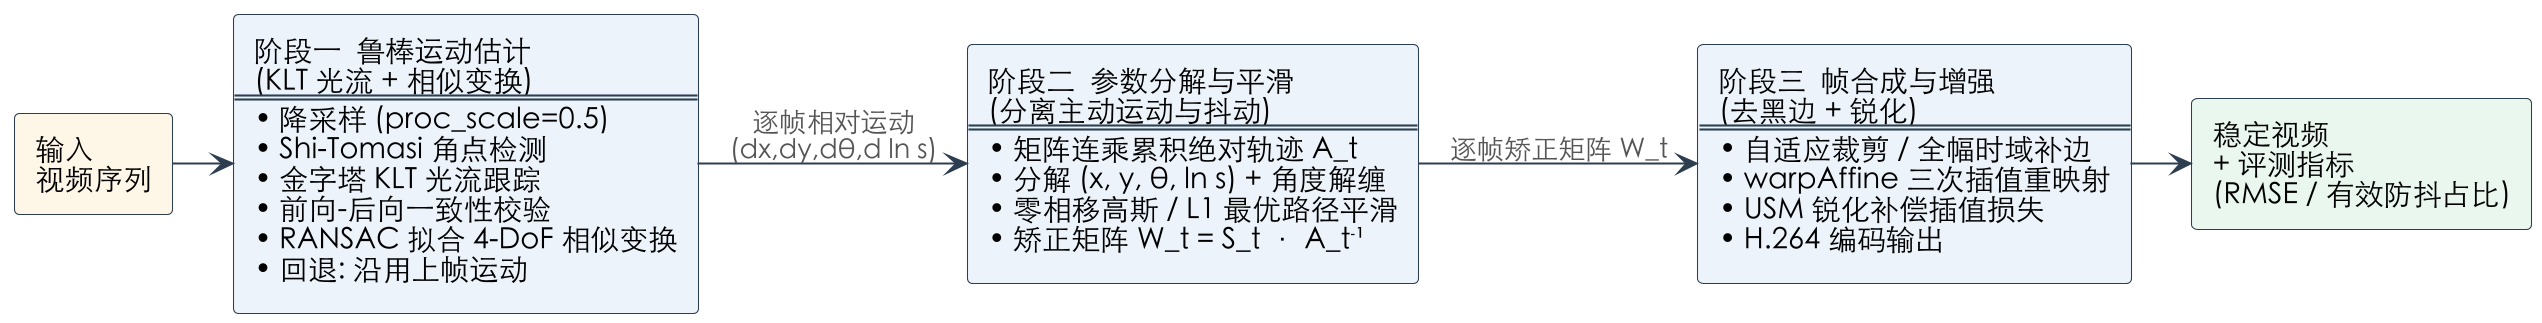
\includegraphics[width=\textwidth]{./image/pipeline_flow.png}
\bicaption[fig:pipeline]{图}{\centering 三阶段视频防抖流水线总体框图}{Fig.}{\centering Overall architecture of the three-stage video stabilization pipeline}
\end{figure*}

\section{基于 KLT 光流的鲁棒运动估计}

在缺乏硬件陀螺仪（Gyroscope）或惯性测量单元（IMU）支持的情况下，视频防抖完全依赖于图像序列的 2D 几何变换来推断摄像机的运动。考虑到本任务需要补偿的主动运动主要是平移、旋转与前后推进（缩放），且 6 自由度仿射变换中的剪切自由度在相机运动下并无物理意义、反而易在噪声下产生画面畸变，本文采用 4 自由度的相似变换（Similarity Transform）模型来描述全局背景运动。相邻帧 $I_{t-1}\!\to\!I_t$ 的相对运动以参数 $(dx, dy, d\theta, d\ln s)$ 表示，分别对应平移、旋转角与缩放的自然对数，其对应的相似变换矩阵为：
\begin{equation}
T_{raw}(t) = \begin{bmatrix} s\cos\theta & -s\sin\theta & dx \\ s\sin\theta & s\cos\theta & dy \\ 0 & 0 & 1 \end{bmatrix}
\end{equation}
将缩放以对数 $d\ln s$ 表示，可使其在后续轨迹平滑中与平移、旋转一样满足加性累积，避免参数相加的近似误差。

\subsection{降采样特征检测与金字塔 KLT 跟踪}
不同于逐帧重新检测并匹配描述子的高开销做法，视频相邻帧之间场景高度连续，更适合采用稀疏光流跟踪。本文首先在当前帧上以 Shi-Tomasi 准则~\cite{shitomasi1994} 检测角点（\texttt{goodFeaturesToTrack}），即保留自相关矩阵 $M$ 的较小特征值 $\min(\lambda_1,\lambda_2)$ 超过阈值的强角点，使被跟踪点天然具有良好的可跟踪性：
\begin{equation}
M = \sum_{w}\begin{bmatrix} I_x^2 & I_xI_y \\ I_xI_y & I_y^2 \end{bmatrix}, \quad R = \min(\lambda_1,\lambda_2)
\end{equation}

随后采用金字塔 Lucas-Kanade（KLT）光流~\cite{lucas1981,bouguet2001} 将这些角点跟踪到下一帧。LK 法在亮度恒定与局部位移一致假设下，于每个角点 $p$ 的邻域 $w$ 内最小化光度残差，求解位移 $\mathbf{d}=(u,v)^T$：
\begin{equation}
\mathbf{d} = \arg\min_{\mathbf{d}} \sum_{x\in w}\big[I_{t-1}(x) - I_t(x+\mathbf{d})\big]^2
\end{equation}
通过构建图像金字塔由粗到细迭代，可在保持小窗口线性近似有效性的同时，覆盖快速摇摄带来的大幅度位移。

为进一步降低 1080P 视频的计算量并增强对运动模糊的鲁棒性，本文在降采样比例 $\rho$（默认 $0.5$）的图像上完成检测与跟踪，所得平移分量再按 $1/\rho$ 缩放回全分辨率（旋转与缩放与图像尺度无关），在实测中既显著提速，又因模糊在低分辨率下被弱化而提升了估计稳定性。

\subsection{前向-后向一致性校验}
KLT 跟踪在遮挡、弱纹理或前景运动处会产生错误的对应。为剔除这类不可靠点，本文引入前向-后向（Forward-Backward）一致性校验~\cite{kalal2010}：将点 $p$ 从 $I_{t-1}$ 正向跟踪到 $I_t$ 得到 $\hat p$，再由 $I_t$ 反向跟踪回 $I_{t-1}$ 得到 $p'$，仅保留回跳误差小于阈值 $\varepsilon$ 的点：
\begin{equation}
\|p - p'\|_2 < \varepsilon
\end{equation}
合法跟踪点的正反向轨迹应当闭合，而错误跟踪点的回跳误差通常很大，故该校验能高效滤除外点。考虑到快速摇摄时合法点的回跳误差也会偏大，阈值取相对宽松的 $\varepsilon=3$ 像素（处理分辨率下），以避免过严而误删有效点。

\subsection{RANSAC 相似变换拟合与回退机制}
经过校验的对应点集中仍可能混杂动态前景对象（如行人、车辆）造成的外点，若直接用最小二乘拟合将被严重带偏。因此本文采用随机抽样一致性（RANSAC）~\cite{ransac1981} 估计相似变换（\texttt{estimateAffinePartial2D}）。RANSAC 每次随机抽取最小子集计算候选模型 $T$，统计重投影误差小于阈值的内点数量，经多次迭代后输出内点支持最多的最优相似变换 $T_{raw}(t)$，从而仅依据静态背景估计摄像机运动。

若当前帧有效跟踪点不足或拟合失败，系统触发回退（Fallback）机制。值得强调的是，本文并不将 $T_{raw}(t)$ 置为单位矩阵——那会在轨迹上引入突变，反而表现为一次人为抖动；而是\textbf{沿用上一帧的相对运动}（常速预测），使轨迹在偶发失败处保持平滑连续，更符合摄像机运动的物理惯性。

\section{运动平滑、帧合成与画面增强}
\subsection{轨迹绝对化与参数分解平滑}
$T_{raw}(t)$ 表示第 $t$ 帧相对于第 $t-1$ 帧的相对变换。为获得全局稳定的效果，需将相对矩阵精确连乘，求取以第一帧为世界坐标系基准的累积绝对轨迹 $A_t$：
\begin{equation}
A_t = T_{raw}(t) \cdot A_{t-1}, \quad A_0 = I
\end{equation}

直接对 $3 \times 3$ 的矩阵元素序列进行一维低通滤波，往往会破坏相似变换的几何约束特性，产生剪切或非法缩放导致的画面畸变。为解决该问题，本文将每一帧的绝对轨迹 $A_t$ 分解到 4 个具有独立物理意义的参数上：水平/垂直平移 $(x_t, y_t)$、旋转角 $\theta_t$ 与对数尺度 $\ell_t=\ln s_t$：
\begin{equation}
(x_t, y_t, \theta_t, \ell_t) = \mathrm{decompose}(A_t)
\end{equation}
其中旋转角 $\theta_t$ 在序列上做解缠（unwrap）处理，以消除 $\pm\pi$ 跳变。在参数空间而非矩阵元素上平滑，可保证平滑后的轨迹仍为合法相似变换，从根本上规避几何畸变。

本文提供两种互补的平滑器对 4 条参数轨迹分别进行处理：

\textbf{（1）零相移高斯低通。} 以标准差 $\sigma$ 的高斯核对每条参数轨迹做低通滤波。为防止普通单向滤波带来的相位滞后（Phase Delay）——即平滑轨迹虽平缓却在时间轴上落后于原轨迹、表现为“防抖慢半拍”——本文采用零相移前向-后向双重滤波。该平滑器简单稳健，作为默认方法。

\textbf{（2）L1 最优相机路径。} 借鉴 Grundmann 等~\cite{grundmann2011} 的思想，将理想相机路径约束为分段的静止、匀速与匀加速运动，通过最小化路径一阶、二阶、三阶差分的 $L1$ 范数加权和求解：
\begin{equation}
\min_{P}\ \omega_1\|D^1P\|_1 + \omega_2\|D^2P\|_1 + \omega_3\|D^3P\|_1
\end{equation}
其中 $P$ 为平滑后参数轨迹，$D^k$ 为 $k$ 阶差分算子。该问题逐通道转化为线性规划求解。$L1$ 范数的稀疏特性使其倾向于产生分段恒定的导数，从而生成更接近专业摄影的“静止—匀速推拉—静止”运镜，能更干净地保留主动运动意图。

设平滑后参数重组得到的理想轨迹矩阵为 $S_t$，则当前帧用于防抖重映射的逐帧矫正矩阵为：
\begin{equation}
W_t = S_t \cdot A_t^{-1}
\end{equation}
该矩阵为图像重采样所需的 dst$\to$src 映射，可直接用于仿射重映射。

\subsection{自适应裁剪与全幅时域运动补边}
对原始帧施加矫正矩阵 $W_t$ 后，画面会因平移、旋转而在边缘露出无像素的黑边。人眼对边缘伪影极为敏感，因此去黑边是帧合成的关键。本文提供两条互补路径。

\textbf{（1）预算约束的自适应中心裁剪。} 对每一帧，通过二分搜索求出令输出矩形四角都落回原图内所需的最小中心放大倍数；取所有帧的高分位数并钳制到预算上限 $z_{\max}$，得到全局统一的放大倍数，从而既藏住黑边又尽量少裁画面。对于个别需放大过大的剧烈帧，引入\textbf{矫正量阻尼}：按比例将该帧矫正向“不矫正”收缩，直到其所需放大恰好落入预算。其物理含义是——剧烈摇摄本就是主动运动，对其少补偿一点以换取全程固定的小裁剪、画面贴近原片且永不露黑边。

\textbf{（2）全幅时域运动补边。} 当不希望损失任何视野与分辨率时，本文借鉴 Matsushita 等~\cite{matsushita2006} 的运动修补思想，用相邻帧的真实像素填补当前帧的黑边空洞。设世界同一点在第 $i$ 帧的稳定画布位置为 $x$，其在第 $j$ 帧源图中的对应采样矩阵为：
\begin{equation}
G_{i\leftarrow j} = A_j \cdot A_i^{-1} \cdot W_i
\end{equation}
按时间距离由近及远遍历邻帧，将其像素经 $G_{i\leftarrow j}$ warp 到当前画布以增量填补空洞（近邻优先，画质更接近），并对“原内容$\leftrightarrow$填充内容”的接缝做窄带羽化柔化；残留的极小空洞最后由图像修补（inpainting）收尾。该路径可在不裁剪的前提下输出全分辨率、全视野、无黑边的稳定画面。

\subsection{锐化增强与输出}
最终画面通过三次插值（Cubic Interpolation）配合矫正矩阵 $W_t$ 完成重映射。由于多次插值会引入轻微的高频损失，本文以非锐化掩模（Unsharp Masking, USM）做温和的锐度补偿：
\begin{equation}
I_{out} = (1+\alpha)\,I - \alpha\, G_{\sigma}\!*\,I
\end{equation}
其中 $G_{\sigma}*I$ 为高斯模糊版本，$\alpha$ 为较柔和的锐化强度（默认 0.6），以避免过锐产生塑料感。增强后的帧以 H.264 编码输出，保证良好的播放兼容性。

\section{实验验证与结果分析}

\subsection{测试数据集与评估指标}
为了精确量化算法的性能表现，本文采用四组在真实图像上附加已知摄像机理论轨迹（Ground Truth）合成的测试视频（每段 335 帧），其逐帧真值平移 $(T_x, T_y)$ 与旋转 $\theta$ 已知：
\begin{itemize}
    \item \textbf{手持步行 (Handheld Walking)}：模拟人手持摄像机行走时典型的周期性晃动与前后仰震荡（含运动模糊）。
    \item \textbf{骑行颠簸 (Bumpy Riding)}：模拟固定在车把上的设备因路面不平带来的高频剧烈冲击抖动（含运动模糊，工况最极端）。
    \item \textbf{画面剧烈抖动 (Severe Camera Shake)}：模拟人为快速转动镜头时的大幅摇摄（无运动模糊）。
    \item \textbf{静止站立 (Static Standing)}：模拟原地持机时的小幅手抖（含运动模糊）。
\end{itemize}

本文从两个互补维度评估算法：

\textbf{（1）运动估计精度}采用均方根误差（RMSE）衡量，即算法估计的累积绝对平移轨迹与 Ground Truth 真值轨迹在 $X$、$Y$ 轴上的像素级偏差，总 RMSE 取二者的几何和。该指标越低，代表运动估计越准确地还原了真实的相机运动。

\textbf{（2）防抖效果}采用\textbf{有效防抖时长占比}衡量。对处理后的视频重新估计逐帧运动，以高斯低通分离出主动运动的低频趋势，残差即为高频抖动；某帧的残余抖动幅度低于阈值（1 像素）即视为“平稳”，平稳帧数占总帧数的比例即为有效防抖时长占比。该指标直接对应肉眼可感知的“画面平稳的时长比例”，并辅以处理前后的平均逐帧抖动幅度（像素）加以佐证。

\begin{figure*}[htbp]
\centering
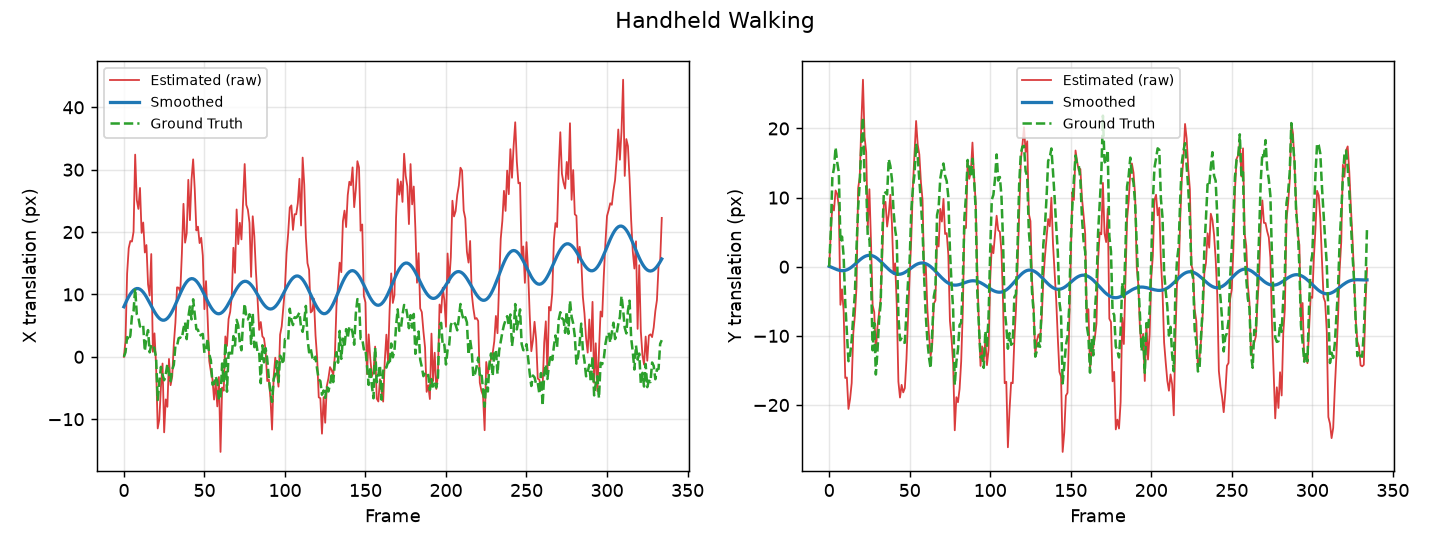
\includegraphics[width=0.92\textwidth]{./image/synth_handheld_walking_trajectory_eval.png}
\bicaption[fig:handheld]{图}{\centering 手持步行场景绝对运动轨迹对比}{Fig.}{\centering Absolute motion trajectory comparison in handheld walking scenario}
\end{figure*}

\subsection{轨迹可视化与量化分析}
将各场景下的累积绝对运动轨迹按 $X$、$Y$ 两个方向随帧序变化进行可视化，每幅图包含算法估计的原始轨迹（红线）、平滑后轨迹（蓝线）以及真值轨迹（绿色虚线）。图\ref{fig:handheld} 展示了最典型的手持步行场景。从图中可清晰地观察到两点：其一，红色的估计原始轨迹与绿色的真值虚线几乎完全重合，且二者都呈现大量锯齿状的高频抖动，这证明本文的 KLT 光流加相似变换估计能够准确还原真实的相机运动；其二，经参数分解与零相移高斯滤波后，蓝色平滑轨迹变得极为平缓，剔除了高频震荡的同时保留了相机平缓移动的低频意图，正是该平滑轨迹被用作防抖重映射的目标位姿。

\begin{figure*}[htbp]
\centering

\includegraphics[width=0.92\textwidth]{./image/synth_bumpy_riding_trajectory_eval.png}
\bicaption[fig:bumpy]{图}{\centering 骑行颠簸场景绝对运动轨迹对比}{Fig.}{\centering Absolute motion trajectory comparison in bumpy riding scenario}
\end{figure*}

图\ref{fig:bumpy} 和图\ref{fig:panning} 分别展示了骑行颠簸和画面剧烈抖动场景下的轨迹评估图。其中画面剧烈抖动场景虽存在大幅摇摄，但因不含运动模糊，红色估计轨迹与绿色真值贴合最紧；而骑行颠簸场景兼有剧烈运动与运动模糊，估计轨迹的偏差相对最大。

\begin{figure*}[htbp]
\centering
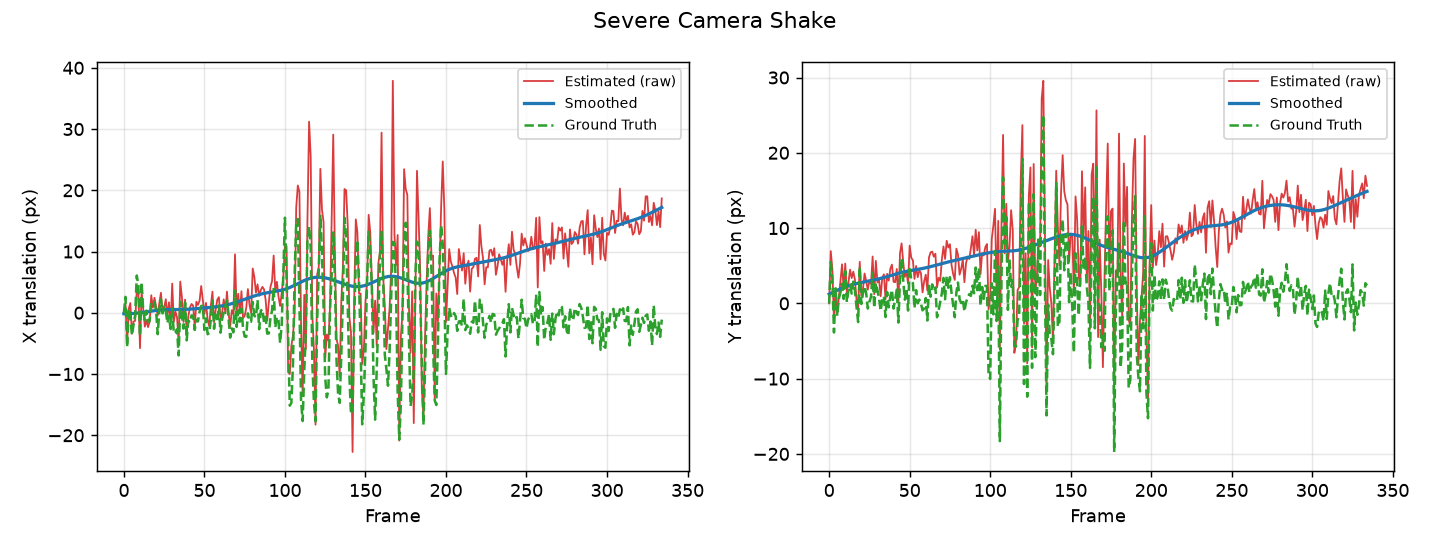
\includegraphics[width=0.92\textwidth]{./image/synth_quick_panning_trajectory_eval.png}
\bicaption[fig:panning]{图}{\centering 画面剧烈抖动场景绝对运动轨迹对比}{Fig.}{\centering Absolute motion trajectory comparison in severe camera shake scenario}
\end{figure*}

各测试场景下，运动估计在 $X$、$Y$ 方向的 RMSE 及总平移 RMSE 统计如表\ref{tab:rmse} 所示。

\begin{table}[htbp]
\centering
\captionnamefont{\xiaowuhao\bf }
\captiontitlefont{\xiaowuhao\bf }
\bicaption[tab:rmse]{表}{不同场景下运动估计的平移均方根误差 (RMSE)}{Table}{Translation RMSE of motion estimation across different scenarios}
\renewcommand\tabcolsep{0.5em}
\resizebox{\columnwidth}{!}{%
\begin{tabular}{cccc}
\toprule
{测试场景} & \makecell{X 轴\\RMSE/px} & \makecell{Y 轴\\RMSE/px} & \makecell{总\\RMSE/px} \\
\midrule
画面剧烈抖动 & 9.78 & 7.92 & 12.59 \\
手持步行 & 14.22 & 6.10 & 15.47 \\
静止站立 & 11.26 & 15.10 & 18.83 \\
骑行颠簸 & 44.18 & 20.38 & 48.66 \\
\bottomrule
\end{tabular}}
\end{table}

表\ref{tab:rmse} 的数据证实：
1) 不含运动模糊的\textbf{画面剧烈抖动}场景虽运动幅度最大，但因图像清晰、跟踪可靠，运动估计精度最高，总 RMSE 仅为 12.59 像素，平均内点率达 1.00。
2) \textbf{手持步行}与\textbf{静止站立}场景取得 15.47 与 18.83 像素的均衡误差，证明算法对日常消费级设备的常见抖动具有良好的泛化能力。
3) 在最严苛的\textbf{骑行颠簸}场景下，剧烈运动与显著运动模糊叠加，超出了 2D 相似变换可完美建模的范畴，误差最高（48.66 像素）；但相比原始抖动，主观上画面可用性仍有明显改善。

为评估实际防抖效果，表\ref{tab:ratio} 进一步给出处理前后的有效防抖时长占比与平均逐帧抖动，并对比两种平滑器的表现。

\begin{table}[htbp]
\centering
\captionnamefont{\xiaowuhao\bf }
\captiontitlefont{\xiaowuhao\bf }
\bicaption[tab:ratio]{表}{处理前后有效防抖时长占比与平均抖动（高斯/L1 平滑）}{Table}{Effective stabilization-time ratio and mean jitter before/after processing (Gaussian/L1)}
\renewcommand\tabcolsep{0.35em}
\resizebox{\columnwidth}{!}{%
\begin{tabular}{ccccc}
\toprule
\multirow{2}{*}{测试场景} & \multicolumn{3}{c}{有效防抖占比 (\%)} & \makecell{抖动/px} \\
\cmidrule(lr){2-4}\cmidrule(lr){5-5}
 & 原始 & 高斯 & L1 & 原始$\to$高斯 \\
\midrule
手持步行 & 0.6 & \textbf{57.6} & 17.9 & 7.39$\to$0.99 \\
画面剧烈抖动 & 1.2 & 56.4 & \textbf{59.4} & 8.93$\to$1.06 \\
静止站立 & 49.0 & 95.5 & \textbf{96.1} & 1.15$\to$0.41 \\
骑行颠簸 & 0.0 & \textbf{1.8} & 0.9 & 67.80$\to$29.75 \\
\bottomrule
\end{tabular}}
\end{table}

由表\ref{tab:ratio} 可见：除极端的骑行颠簸工况外，算法将有效防抖时长占比从处理前的 0.6\%--49\% 大幅提升至 56\%--96\%，平均逐帧抖动由 7--9 像素降至约 1 像素，画面平稳性获得质的飞跃。两种平滑器各有所长：\textbf{零相移高斯}总体更稳健，尤其在抖动随机性强的手持步行场景显著优于 L1（57.6\% vs.\ 17.9\%），适合作为默认方法；\textbf{L1 最优路径}凭借分段恒速的路径约束，在含明显主动运镜的画面剧烈抖动与静止站立场景下略胜一筹，更利于保留摄影意图。骑行颠簸因运动幅度远超裁剪预算所能补偿的范围，两种方法均仅能部分改善，构成本文方法在 2D 模型下的能力边界。

在运行效率方面，运动估计阶段（含前向-后向校验）平均约 3--7\,ms/帧，全部 335 帧的整段处理在普通 CPU 上仅需数秒，且全程无估计失败回退帧、平均内点率达 0.95--1.00，验证了流水线良好的实时性与鲁棒性。

\section{结\quad 论}
针对视频序列中高频不规则抖动的难题，本文摒弃了可靠性不足的自研实现，基于 OpenCV 高效后端构建了一套不依赖深度学习、可近实时运行的三阶段视频防抖流水线。本文得出以下主要结论：

1) 以降采样金字塔 KLT 光流替代逐帧重检测匹配，辅以前向-后向一致性校验与 RANSAC 相似变换拟合，并在估计失败时沿用上帧运动而非置单位阵，是保证 4 自由度运动估计精准、连续、抗动态外点的根基；实验中平均内点率达 0.95--1.00、无回退帧，运动估计总 RMSE 低至 12.59 像素。

2) 将绝对轨迹分解到平移、旋转角与对数尺度参数空间后再平滑，能从根本上规避直接矩阵插值导致的几何畸变；零相移高斯与 L1 最优路径两种平滑器互补——前者更稳健、后者更利于保留运镜意图，可按场景灵活选用。

3) 提出预算约束的自适应中心裁剪与全幅时域运动补边两条去黑边路径，配合 USM 锐化，在不依赖去模糊的前提下输出贴近原片、无黑边的稳定画面；除极端骑行颠簸外，有效防抖时长占比由处理前的 0.6\%--49\% 提升至 56\%--96\%。

综上所述，本文方法有效提升了受扰动视频序列的时空稳定性，其参数分解平滑与双路径去黑边策略兼具理论参考价值与工程实用意义。后续研究可考虑引入网格形变（Grid Warping）以建模视差与卷帘快门（Rolling Shutter）效应，进一步逼近影视级防抖水平。


\bibliographystyle{unsrt}
\bibliography{ref}

\end{document}
